\documentclass[a4paper,12pt]{article}

% --- Базовые пакеты ---
\usepackage[russian]{babel}
\usepackage[T2A]{fontenc}
\usepackage[utf8]{inputenc}
\usepackage{geometry}
\usepackage{amsmath, amssymb}
\usepackage{graphicx}
\usepackage{cancel}
\usepackage{float} 
\usepackage{xcolor}
\usepackage{array}
\usepackage{caption}
\usepackage{booktabs}
\usepackage{subcaption}
\usepackage{pgfplots}
\pgfplotsset{compat=1.18}
\usetikzlibrary{arrows.meta, matrix, positioning}
\usepackage{capt-of}
\usepackage{multirow}
\usepackage[siunitx]{circuitikz}
\usepackage[bottom]{footmisc}
\usepackage{tcolorbox}
\usepackage{nicematrix}
\usepackage{tikz}

% --- Гиперссылки (ОДИН РАЗ!) ---
\usepackage{hyperref}
\hypersetup{
	colorlinks=true,
	linkcolor=red,
	citecolor=red,
	urlcolor=red,
	filecolor=red,
	linktoc=page
}

% --- Содержание ---
\usepackage{tocloft}
\usepackage{etoolbox}

% Патчим \tableofcontents для черного текста и красных номеров страниц
\preto\tableofcontents{%
	\begingroup
	\renewcommand{\contentsline}[4]{%
		\ifnum\pdfstrcmp{##1}{section}=0
		\vskip 4pt{\normalfont\color{black}##2}\nobreak\hfill
		{\normalfont\color{red}\hyperlink{##4}{##3}}\par
		\else\ifnum\pdfstrcmp{##1}{subsection}=0
		\vskip 2pt\hspace{1.5em}{\normalfont\color{black}##2}\nobreak\hfill
		{\normalfont\color{red}\hyperlink{##4}{##3}}\par
		\else
		\vskip 1pt\hspace{3em}{\normalfont\color{black}##2}\nobreak\hfill
		{\normalfont\color{red}\hyperlink{##4}{##3}}\par
		\fi\fi
	}%
}
\appto\tableofcontents{\endgroup}

% --- Листинги MATLAB ---
\usepackage{listings}
\usepackage{matlab-prettifier} % <-- Подключаем пакет

% Цвета
\definecolor{codebg}{RGB}{250,250,252}
\definecolor{linenumcolor}{RGB}{150,150,170}
\definecolor{matlabblue}{RGB}{0,0,200}
\definecolor{matlabgreen}{RGB}{30,130,30}
\definecolor{matlaborange}{RGB}{200,80,0}

% Настройка matlab-prettifier (НЕ через \lstset{style=...})
\lstset{
	style              = Matlab-editor, % Стиль пакета
	basicstyle         = \mlttfamily\small, % ВАЖНО: шрифт из пакета
	backgroundcolor    = \color{codebg},
	frame              = single,
	frameround         = tttt,
	framesep           = 4pt,
	rulecolor          = \color{matlabblue!30},
	numbers            = left,
	numberstyle        = \tiny\color{linenumcolor},
	numbersep          = 10pt,
	breaklines         = true,
	tabsize            = 4,
	showstringspaces   = false,
	captionpos         = b,
	xleftmargin        = 15pt,
	xrightmargin       = 5pt,
	escapeinside       = {\%*}{*)},
}

% Настройки подписей листингов
\renewcommand{\lstlistingname}{Листинг}
\DeclareCaptionFormat{redlisting}{#1\textcolor{red}{#2}#3}
\captionsetup[lstlisting]{format=redlisting}

% --- Геометрия и общие настройки ---
\geometry{left=1.5cm, right=2cm, bottom=2cm, top=2cm}
\captionsetup[figure]{name=Рисунок}
\captionsetup[table]{name=Таблица}
\captionsetup{labelsep=endash}
\newcommand{\figwidth}{0.5\textwidth}


\begin{document}
	
	\begin{titlepage}
		\centering
		
		\vspace*{0.5cm}
		{\small
			Министерство науки и высшего образования Российской Федерации\\[2pt]
			Федеральное государственное автономное образовательное учреждение\\
			высшего образования\\[2pt]
			\textbf{«Национальный исследовательский университет ИТМО»}\\
		}
		
		\vspace{0.8cm}
		\hrule height 0.8pt
		\vspace{0.3cm}
		
		{\large Факультет систем управления и робототехники}
		
		\vspace{0.3cm}
		\hrule height 0.4pt
		\vspace{2.5cm}
		
		{\Huge\bfseries ОТЧЁТ}\\[0.4cm]
		{\LARGE\bfseries о лабораторной работе №3}\\[0.8cm]
		
		\begin{tcolorbox}[
			colback=gray!4,
			colframe=gray!10,
			boxrule=0.8pt,
			arc=4pt,
			left=12pt, right=12pt, top=8pt, bottom=8pt
			]
			\centering
			{\large По дисциплине:\\[4pt]}
			{\large\bfseries «Нелинейные системы управления»}\\[10pt]
		\end{tcolorbox}
		
		\vspace{5cm}
		
		\begin{minipage}{0.45\textwidth}
			\raggedright
			{\large\bfseries Студенты:}\\[4pt]
			Охрименко Е.\,Д.\\
			Титаренко П. А.
		\end{minipage}
		\hfill
		\begin{minipage}{0.45\textwidth}
			\raggedleft
			{\large\bfseries Преподаватель:}\\[4pt]
			Зименко К. А.\\
		\end{minipage}
		
		\vfill
		\vspace{0.4cm}
		{\large Санкт-Петербург, 2026}
	\end{titlepage}
	
	\newpage
	\tableofcontents
	
	
	\newpage \section{Анализ линеаризуемости системы}
	



Рассмотрим систему:

\begin{equation}
	\begin{cases}
		\dot{x}_1 = -x_1 + x_2 - x_3 \\
		\dot{x}_2 = -x_1 x_3 - x_2 + u \\
		\dot{x}_3 = -x_1 + u \\
		y = x_3
	\end{cases}
\end{equation}

\subsection{Проверка линеаризуемости и нахождение относительной степени}

Для определения относительной степени $\rho$ продифференцируем выход $y = x_3$ по времени до появления управления $u$:
$$ \dot{y} = \dot{x}_3 = -x_1 + u. $$

Так как управление $u$ появилось уже в первой производной с коэффициентом $1 \neq 0$, относительная степень системы:
$$ \rho = 1$$

Поскольку $\rho = 1$ определена во всем пространстве состояний $\mathbb{R}^3$ и не зависит от координат, система является глобально линеаризуемой по входу-выходу.


\subsection{Нормальная форма системы}

Для построения нормальной формы введем новые координаты. Так как относительная степень $\rho=1$ а размерность системы $n=3$ то необходимо найти две внутренние координаты $\eta_1$ и $\eta_2$. Они должны удовлетворять условию независимости от управления $L_g \eta_i = 0$. Для вектора поля управления $g(x)=[0 \ 1 \ 1]^T$ это условие записывается как
$$ \frac{\partial \eta}{\partial x_2} + \frac{\partial \eta}{\partial x_3} = 0 $$

Выберем следующие функции в качестве внутренних координат
$$ \eta_1 = x_2 - x_3 $$
$$ \eta_2 = x_1 $$

Внешняя координата соответствует выходу системы
$$ \xi_1 = y = x_3 $$

Теперь найдем производные новых координат по времени. Для внешней координаты при выборе линеаризующего управления $u = x_1 + v$ получаем
$$ \dot{\xi}_1 = \dot{x}_3 = -x_1 + u = -x_1 + (x_1 + v) = v $$

Для первой внутренней координаты вычислим производную
$$ \dot{\eta}_1 = \dot{x}_2 - \dot{x}_3 = (-x_1 x_3 - x_2 + u) - (-x_1 + u) = -x_1 x_3 - x_2 + x_1 $$

Выразим старые переменные через новые используя соотношения $x_1=\eta_2$ и $x_3=\xi_1$ и $x_2=\eta_1+\xi_1$. Подставим их в выражение для $\dot{\eta}_1$
$$ \dot{\eta}_1 = -\eta_2 \xi_1 - (\eta_1 + \xi_1) + \eta_2 = -\eta_1 - \xi_1 + \eta_2(1 - \xi_1) $$

Для второй внутренней координаты производная равна
$$ \dot{\eta}_2 = \dot{x}_1 = -x_1 + x_2 - x_3 $$

Подставим замены переменных
$$ \dot{\eta}_2 = -\eta_2 + (\eta_1 + \xi_1) - \xi_1 = \eta_1 - \eta_2 $$

Итоговая нормальная форма системы имеет вид
\begin{equation}
	\begin{cases}
		\dot{\xi}_1 = v \\
		\dot{\eta}_1 = -\eta_1 - \xi_1 + \eta_2(1 - \xi_1) \\
		\dot{\eta}_2 = \eta_1 - \eta_2
	\end{cases}
\end{equation}

Область определения преобразования -- это множество точек $x$, в котором замена координат $z = T(x)$ является диффеоморфизмом. Проверим,  является ли система с замененными координатами диффеоморфизмом. Вычислим определитель матрицы Якоби преобразования (листинг~\ref{lst:J}):
$$ J_T(x) = \frac{\partial z}{\partial x} = \begin{bmatrix} 
	0 & 0 & 1 \\ 
	0 & 1 & -1 \\ 
	1 & 0 & 0 \end{bmatrix} $$

Определитель данной матрицы равен:
$$ \det(J_T) = -1 $$

Так как $\det(J_T) = -1 \neq 0$ во всех точках пространства состояний и так как коэффициент при управлении в первой производной выхода равен единице, преобразование $T(x)$ является глобальным диффеоморфизмом. Следовательно, нормальная форма определена во всем пространстве $\mathbb{R}^3$.


\subsection{Проверка минимальной фазовости}

Система является минимально-фазовой, если её нуль-динамика асимптотически устойчива. Нуль-динамика описывает поведение внутренних координат при условии $\xi_1 = 0$. Подставим $\xi_1 = 0$ в уравнения внутренней динамики:
\begin{equation}
	\begin{cases}
		\dot{\eta}_1 = -\eta_1 + \eta_2 \\
		\dot{\eta}_2 = \eta_1 - \eta_2
	\end{cases}
\end{equation}

Матрица коэффициентов полученной линейной системы имеет вид:
$$ A_0 = \begin{bmatrix} -1 & 1 \\ 1 & -1 \end{bmatrix} $$

Характеристическое уравнение: $$\det(A_0 - \lambda I) = \lambda(\lambda + 2) = 0$$ имеет корни $\lambda_1 = 0$ и $\lambda_2 = -2$. Наличие нулевого собственного числа означает, что нуль-динамика не является асимптотически устойчивой. Следовательно, исходная система не является минимально-фазовой.


\section{Синтез стабилизирующего управления}

Рассмотрим систему:
\begin{equation}
	\begin{cases}
		\dot{x}_1 = -x_1 + x_2 \\
		\dot{x}_2 = x_1 - x_2 - x_1 x_3 + u \\
		\dot{x}_3 = x_1 + x_1 x_2 - 2x_3
	\end{cases}
\end{equation}

\subsection{Линеаризация обратной связью}
Так как управление $u$ входит линейно во второе уравнение, выберем выход системы $y = x_2$. Относительная степень данной системы $\rho = 1$. Продифференцируем выход по времени:
$$ \dot{y} = \dot{x}_2 = x_1 - x_2 - x_1 x_3 + u $$
Для компенсации нелинейности $-x_1 x_3$ и приведения внешней динамики к линейному виду $\dot{y} = v$, выберем закон управления:
$$ u = x_1 x_3 + v $$
Подставляя это выражение в исходную систему, получаем замкнутую систему с линейной подсистемой $(x_1, x_2)$:
\begin{equation}
	\begin{cases}
		\dot{x}_1 = -x_1 + x_2 \\
		\dot{x}_2 = x_1 - x_2 + v \\
		\dot{x}_3 = -2x_3 + x_1(1 + x_2)
	\end{cases}
\end{equation}

\subsection{Синтез регулятора}
Запишем линеаризованную часть системы в матричном виде:

\[
\dot x = \begin{bmatrix}
	-1 & 1 \\
	1 & -1
\end{bmatrix} x + \begin{bmatrix}
0 \\ 1
\end{bmatrix} v
\]

Синтезируем матрицу управления:

\[u = -Kx\] для желаемого спектра:

\[\sigma(\Gamma)\left\{-3 ; -4\right\}\]
по формуле аккермана (листинг~\ref{lst:acker}). Получаем:

\[K = \begin{bmatrix}
	7 & 5
\end{bmatrix}\]

При проверке собственных чисел спкетр совпал с желаемым, матрица найдена верно.

\subsection{Анализ устойчивости}
При выбранном управлении переменные $x_1$ и $x_2$ стремятся к нулю экспоненциально. Уравнение для $x_3$ представляет собой устойчивую линейную систему $\dot{x}_3 = -2x_3$ с возмущением $x_1(1+x_2)$. Поскольку возмущение затухает вместе с $x_1$ и $x_2$, переменная $x_3$ также асимптотически стремится к нулю. Следовательно, начало координат всей системы глобально асимптотически устойчиво. 

Промоделируем нелинейную систему с регулятором для линеаризованной части при: \[x(0) = \begin{bmatrix}
-1\\-2\\-3
\end{bmatrix}\]
 получим, что траектории компонент асимптотически устойчивы.

\begin{figure}[H]
	\centering
	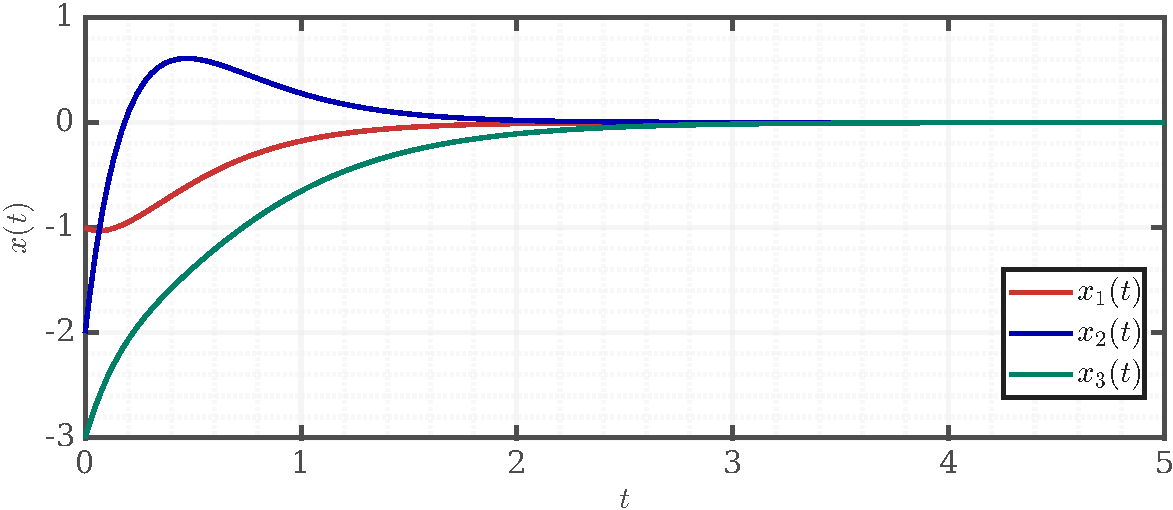
\includegraphics[width=0.8\textwidth]{../images/x_sys_2.pdf}
	\caption{Вектор \(x(t)\) замкнутой нелинейной системы}
\end{figure}




\newpage \section{Анализ неминимально-фазовой системы}

Рассмотрим систему:
\begin{equation}
	\begin{cases}
		\dot{x}_1 = x_2 \\
		\dot{x}_2 = -x_1 + x_3 + u \\
		\dot{x}_3 = x_3 + x_1^2 \\
		y = x_1
	\end{cases}
\end{equation}

\subsection{Линеаризация по входу-выходу}
Для определения относительной степени $\rho$ продифференцируем выход $y=x_1$ до появления управления $u$:
$$ \dot{y} = \dot{x}_1 = x_2 $$
$$ \ddot{y} = \dot{x}_2 = -x_1 + x_3 + u $$
Управление появилось во второй производной с коэффициентом $1 \neq 0$. Следовательно, относительная степень системы $\rho = 2$.
Для линеаризации внешней динамики ($\ddot{y}=v$) выберем закон управления:
$$ u = x_1 - x_3 + v $$

\subsection{Нормальная форма системы}

Так как $n=3$ и $\rho=2$, требуется одна внутренняя координата $\eta$. Внешние координаты:
\[
\xi_1 = x_1 \qquad \xi_2 = x_2
\]

Внутреннюю координату находим из условия $L_g \eta = 0$. Для $g(x)=[0, 1, 0]^T$:
\[
\frac{\partial \eta}{\partial x_2} = 0 \implies \eta = x_3
\]

Якобиан преобразования $z=[x_3, x_1, x_2]^T$ имеет определитель $\det(J_T)=1 \neq 0$, следовательно замена является глобальным диффеоморфизмом.

Продифференцируем новые координаты. При управлении $u = x_1 - x_3 + v$ внешняя динамика линеаризуется:
\begin{align*}
	\dot{\xi}_1 &= \xi_2 \\
	\dot{\xi}_2 &= -x_1 + x_3 + (x_1 - x_3 + v) = v
\end{align*}
Для внутренней координаты, используя $\dot{x}_3 = x_3 + x_1^2$, получаем:
\[
\dot{\eta} = \eta + \xi_1^2
\]
Итоговая нормальная форма:
\[
\begin{cases}
	\dot{\xi}_1 = \xi_2 \\
	\dot{\xi}_2 = v \\
	\dot{\eta} = \eta + \xi_1^2
\end{cases}
\]

\subsection{Нуль-динамика и минимальная фазовость}
Нуль-динамика описывает поведение внутренней координаты при условии поддержания выхода на нуле ($\xi_1 = 0, \xi_2 = 0$). Подставив $\xi_1=0$ в уравнение для $\dot{\eta}$, получаем:
$$ \dot{\eta} = \eta $$
Характеристическое уравнение системы имеет вид: $$\lambda - 1 = 0$$
откуда следует единственное собственное число $\lambda = 1$.
Так как $\text{Re}(\lambda) > 0$, нуль-динамика неустойчива. Следовательно, исходная система не является минимально-фазовой.

	
	
	
\newpage \section{Анализ нелинейной системы}

Рассмотрим систему:
\begin{equation}
	\begin{cases}
		\dot{x}_1 = x_2 \\
		\dot{x}_2 = -x_1 + x_3 u \\
		\dot{x}_3 = -x_3 + u \\
		y = x_1
	\end{cases}
\end{equation}

\subsection{Производные Ли и относительная степень}
Вычислим необходимые производные Ли для выхода $h(x)=x_1$. Векторы полей системы имеют вид $f(x)=[x_2, -x_1, -x_3]^T$ и $g(x)=[0, x_3, 1]^T$.
Градиент выхода $\frac{\partial h}{\partial x} = [1, 0, 0]$.

Первая производная по времени:
\[ L_f h(x) = \frac{\partial h}{\partial x} f(x) = x_2, \quad L_g h(x) = \frac{\partial h}{\partial x} g(x) = 0 \]
Так как $L_g h(x) = 0$, дифференцируем далее. Вторая производная:
\[ L_f^2 h(x) = \frac{\partial (x_2)}{\partial x} f(x) = -x_1 \]
\[ L_g L_f h(x) = \frac{\partial (x_2)}{\partial x} g(x) = x_3 \]
Управление $u$ появляется во второй производной с коэффициентом $x_3$. Следовательно, относительная степень системы $\rho=2$.
Область определения относительной степени определяется условием $L_g L_f h(x) \neq 0$:
\[ D_\rho = \{ x \in \mathbb{R}^3 \mid x_3 \neq 0 \} \]

\subsection{Внутренняя координата и диффеоморфизм}
Покажем, что $\eta = x_2 - \frac{1}{2}x_3^2$ может служить внутренней координатой. Для этого проверим условие инвариантности $L_g \eta = 0$.
Градиент функции $\eta$ равен $\frac{\partial \eta}{\partial x} = [0, 1, -x_3]$. Вычислим производную Ли:
\[ L_g \eta = \begin{bmatrix} 0 & 1 & -x_3 \end{bmatrix} \begin{bmatrix} 0 \\ x_3 \\ 1 \end{bmatrix} = x_3 - x_3 = 0 \]
Условие выполнено, управление не входит в динамику $\eta$ явно.

Для проверки корректности замены координат вычислим якобиан преобразования $T(x) = [\eta, y, \dot{y}]^T = [x_2 - 0.5x_3^2, x_1, x_2]^T$:
\[ J_T(x) = \frac{\partial T}{\partial x} = \begin{bmatrix} 0 & 1 & -x_3 \\ 1 & 0 & 0 \\ 0 & 1 & 0 \end{bmatrix} \]
Определитель матрицы Якоби равен $\det(J_T) = -x_3$. Преобразование является локальным диффеоморфизмом в области $D_T = \{ x \in \mathbb{R}^3 \mid x_3 \neq 0 \}$, которая совпадает с областью определения относительной степени.

\subsection{Нормальная форма и нуль-динамика}
В новых координатах $\xi_1=x_1, \xi_2=x_2, \eta=x_2-0.5x_3^2$ внешняя динамика линеаризуется управлением $u=(\xi_1+v)/x_3$:
\[ \dot{\xi}_1 = \xi_2, \quad \dot{\xi}_2 = v \]
Динамика внутренней координаты находится дифференцированием $\eta$ по времени:
\[ \dot{\eta} = \dot{x}_2 - x_3\dot{x}_3 = (-x_1+x_3u) - x_3(-x_3+u) = -x_1 + x_3^2 \]
Выражая старые переменные через новые ($x_1=\xi_1$, $x_3^2 = 2(\xi_2-\eta)$), получаем уравнение внутренней динамики:
\[ \dot{\eta} = -2\eta + 2\xi_2 - \xi_1 \]
Нуль-динамика соответствует случаю поддержания выхода на нуле ($\xi_1=0, \xi_2=0$):
\[ \dot{\eta} = -2\eta \]
Характеристическое уравнение $\lambda+2=0$ имеет корень $\lambda=-2 < 0$. Поскольку нуль-динамика асимптотически устойчива, исходная система является минимально-фазовой.
	
	
	
\newpage \section{Полная линеаризация обратной связью}

Рассмотрим систему:
\begin{equation}
	\begin{cases}
		\dot{x}_1 = x_2 \\
		\dot{x}_2 = x_3 + x_1^2 \\
		\dot{x}_3 = -x_1 x_2 + (1 + x_1^2)u \\
		y = x_1
	\end{cases}
\end{equation}

\subsection{Относительная степень и новые координаты}
Для определения относительной степени $\rho$ продифференцируем выход $y=x_1$ до появления управления $u$:
\[ \dot{y} = x_2 \]
\[ \ddot{y} = \dot{x}_2 = x_3 + x_1^2 \]
\[ y^{(3)} = \dot{x}_3 + 2x_1\dot{x}_1 = -x_1 x_2 + (1+x_1^2)u + 2x_1 x_2 = x_1 x_2 + (1+x_1^2)u \]
Управление появилось в третьей производной. Коэффициент $\beta(x) = 1+x_1^2 \ge 1 \neq 0$ всюду.
Следовательно, относительная степень системы \textbf{$\rho = 3$}.

Введем новые координаты $z$:
\[ z_1 = y = x_1 \]
\[ z_2 = \dot{y} = x_2 \]
\[ z_3 = \ddot{y} = x_3 + x_1^2 \]

\subsection{Линеаризующая обратная связь}
Требуется привести систему к виду цепочки интеграторов $\dot{z}_3 = v$.
Из выражения для $y^{(3)}$ имеем:
\[ v = x_1 x_2 + (1+x_1^2)u \]
Выразим отсюда управление $u = \alpha(x) + \beta(x)v$:
\[ u = \frac{-x_1 x_2}{1+x_1^2} + \frac{1}{1+x_1^2}v \]

\subsection{Синтез линейного регулятора}

Линеаризованная система в координатах $z$ имеет каноническую форму управляемости:
\[
A = \begin{bmatrix} 0 & 1 & 0 \\ 0 & 0 & 1 \\ 0 & 0 & 0 \end{bmatrix}, \quad 
B = \begin{bmatrix} 0 \\ 0 \\ 1 \end{bmatrix}
\]
Необходимо выбрать управление $v = -Kz$, обеспечивающее размещение полюсов замкнутой системы в точках $\{-2, -2, -3\}$. Матрица регулятора $K$ рассчитана методом Аккермана(листинг~\ref{lst:task5_acker}):
\[
K = \begin{bmatrix} 12 & 16 & 7 \end{bmatrix}
\]
Закон управления для вспомогательного входа принимает вид:
\[
v = -12z_1 - 16z_2 - 7z_3
\]

\subsection{Итоговое управление}
Подставим выражение для $v$ и вернемся к исходным координатам ($z_1=x_1, z_2=x_2, z_3=x_3+x_1^2$):
\[ v = -12x_1 - 16x_2 - 7(x_3 + x_1^2) = -7x_1^2 - 12x_1 - 16x_2 - 7x_3 \]
Окончательный закон управления в исходных координатах:
\[ u(x) = \frac{-x_1 x_2 - 7x_1^2 - 12x_1 - 16x_2 - 7x_3}{1 + x_1^2} \]	
	
\newpage \section{Вывод}
В ходе работы исследованы методы линеаризации обратной связью и построены нормальные формы для нелинейных систем с различной относительной степенью. Синтезированы стабилизирующие управления методом размещения полюсов, а также проанализирована минимальная фазовость через устойчивость нуль-динамики.
	
	
	
	
	
	
	
	
	
	
	
	
	\newpage
	\section{Приложение}
	
	\subsection*{Задание 1}
	
	
\begin{lstlisting}[
style = Matlab-editor, 
caption={Якобиан системы}, 
label={lst:J}
]	
clc; clear;


syms x1 x2 x3

z = [x3;
x2 - x1;
x1];

J = jacobian(z, [x1, x2, x3])

det_J = det(J)	
\end{lstlisting}
	
\begin{lstlisting}[
	style = Matlab-editor, 
	caption={Синтез матрицы регулятора \(K\) методом аккермана}, 
	label={lst:acker}
	]	
clc; clear;

A = [-1 1 ; 1 -1]

B = [0 ; 1]

eig(A)

gamma = [-3; -4]

K = acker(A, B, gamma)

eig(A-B*K)
\end{lstlisting}
	
\begin{lstlisting}[
	style = Matlab-editor, 
	caption={Синтез матрицы регулятора \(K\) методом аккермана}, 
	label={lst:task5_acker}
	]	
clc; clear;

A = [0 1 0; 0 0 1; 0 0 0];

B = [0 ; 0 ; 1];

eig(A)

gamma = [-2; -2; -3]

K = acker(A, B, gamma)

eig(A-B*K)
\end{lstlisting}
	
	
	
\end{document}